\subsection{Segmentación de Imágenes}
La segmentación de imágenes es el proceso de dividir una imagen en diferentes partes o regiones, con el objetivo de simplificar la representación de la imagen y hacerla más significativa y fácil de analizar. Este proceso es fundamental en aplicaciones de visión por computadora, especialmente en la detección de características morfológicas de la piel, como arrugas, poros y manchas \cite{autor2020segmentacion}.

\subsection{Características Morfológicas de la Piel}
Las características morfológicas de la piel son importantes para la evaluación de la salud y la estética facial. En este estudio, se consideran tres características clave:

\subsubsection{Arrugas}
Las arrugas son pliegues o líneas en la piel que se desarrollan debido al envejecimiento, expresiones faciales repetitivas y factores externos. La segmentación de arrugas permite su análisis detallado en el contexto de estudios dermatológicos y cosméticos \cite{autor2021arrugas}.

\subsubsection{Poros}
Los poros son pequeñas aberturas en la piel a través de las cuales las glándulas sebáceas secretan aceites. La identificación y análisis de los poros en imágenes faciales son útiles en la evaluación de problemas de piel, como el acné y la textura de la piel \cite{autor2020poros}.

\subsubsection{Manchas}
Las manchas son áreas de la piel que presentan una pigmentación diferente debido a factores como la exposición al sol o condiciones dermatológicas. La segmentación de manchas es útil para el diagnóstico temprano de condiciones como el melasma o el daño solar \cite{autor2019manchas}.

\subsection{Redes Neuronales Convolucionales (CNN)}
Las Redes Neuronales Convolucionales (CNN) son un tipo de red neuronal que ha demostrado ser eficaz en tareas de procesamiento de imágenes. Estas redes están compuestas por diferentes tipos de capas que permiten extraer características de las imágenes \cite{autor2022cnn}.

\subsubsection{Capas Convolucionales}
Las capas convolucionales son la base de las CNN y se encargan de aplicar filtros sobre la imagen para extraer características relevantes. Estas capas permiten detectar bordes, texturas y otros patrones en las imágenes \cite{autor2021conv}.

\subsubsection{Capas de Activación}
Las capas de activación, como la función ReLU, añaden no linealidad al modelo y permiten que la red capture patrones complejos. Esto es fundamental para mejorar la precisión de la segmentación \cite{autor2020relu}.

\subsubsection{Capas de Pooling (Max Pooling / Average Pooling)}
Las capas de pooling, como el Max Pooling o el Average Pooling, reducen la dimensionalidad de las características extraídas, lo que ayuda a reducir la complejidad computacional y a generalizar mejor el modelo \cite{autor2019pooling}.

\subsubsection{Capas Completamente Conectadas (Fully Connected Layers)}
Estas capas conectan todas las neuronas de una capa con todas las neuronas de la siguiente, permitiendo la integración de las características extraídas y facilitando la clasificación \cite{autor2021fc}.

\subsubsection{Capa de Salida}
La capa de salida de una CNN es responsable de proporcionar el resultado final, que en segmentación de imágenes puede ser un mapa de segmentos o la clasificación de una región específica \cite{autor2022output}.

\subsection{Modelos de Segmentación}
Existen varios modelos de segmentación basados en redes neuronales que son populares en el análisis de imágenes médicas y dermatológicas:

\subsubsection{U-Net}
U-Net es una arquitectura ampliamente utilizada en segmentación médica que permite segmentar características en imágenes con alta precisión \cite{autor2020unet}.

\subsubsection{Fully Convolutional Network (FCN)}
Las Fully Convolutional Networks (FCN) convierten una red completamente conectada en una red convolucional, permitiendo la segmentación en píxeles en lugar de clasificaciones generales \cite{autor2019fcn}.

\subsubsection{SegNet}
SegNet es una arquitectura diseñada para segmentación semántica en tiempo real. Utiliza una estructura de codificación-decodificación para segmentar imágenes \cite{autor2021segnet}.

\subsubsection{Mask R-CNN}
Mask R-CNN extiende la arquitectura Faster R-CNN para incluir la segmentación de objetos en instancias específicas dentro de la imagen \cite{autor2022maskrcnn}.

\subsubsection{DeepLab (v3, v3+)}
DeepLab es una serie de modelos que utilizan convoluciones atrous para mejorar la segmentación en alta resolución \cite{autor2021deeplab}.

\subsection{Métricas de Evaluación}
Las métricas de evaluación son fundamentales para medir la precisión y eficacia de los modelos de segmentación de imágenes:

\subsubsection{Índice de Sorensen-Dice (Dice Coefficient)}
El índice de Dice mide la similitud entre dos conjuntos de datos segmentados, siendo útil en la comparación entre la segmentación automática y la segmentación de referencia \cite{autor2020dice}.

\subsubsection{Coeficiente de Jaccard (Intersection over Union, IoU)}
El coeficiente de Jaccard o IoU es una métrica que evalúa la superposición entre el segmento predicho y el real \cite{autor2021iou}.

\subsubsection{Precisión (Precision)}
La precisión es la relación entre verdaderos positivos y el total de elementos predichos como positivos, lo que refleja la efectividad del modelo en evitar falsos positivos \cite{autor2019precision}.

\subsubsection{Entropía Cruzada (Cross-Entropy)}
La entropía cruzada mide la disonancia entre las distribuciones de probabilidad del modelo y las etiquetas reales \cite{autor2022crossentropy}.

\subsection{Redes de Atención}
Las redes de atención han surgido como un avance significativo en la segmentación de imágenes, permitiendo que el modelo se enfoque en regiones específicas:

\subsubsection{Mecanismo de Atención}
El mecanismo de atención permite a la red asignar diferentes pesos a distintas partes de la imagen para enfocarse en características relevantes \cite{autor2021atencion}.

\subsubsection{Atención Espacial}
La atención espacial asigna pesos basados en la ubicación espacial, destacando áreas específicas en la imagen \cite{autor2020spa}.

\subsubsection{Atención de Canal}
La atención de canal da importancia a las características específicas dentro de los canales de una imagen \cite{autor2019canal}.

\subsubsection{Beneficios de las Redes de Atención}
Las redes de atención mejoran la precisión y eficiencia en la segmentación de imágenes complejas \cite{autor2021beneficios}.

\subsubsection{Ejemplos de Modelos con Atención}
Modelos como Transformer y SENet utilizan mecanismos de atención para mejorar la precisión en tareas de segmentación \cite{autor2022transformer}.

\subsection{Redes Generativas Adversariales (GANs)}
Las GANs son redes compuestas por un generador y un discriminador que compiten entre sí para generar resultados de alta calidad.

\subsubsection{Estructura de GANs (Generador y Discriminador)}
El generador intenta crear datos realistas, mientras que el discriminador evalúa la autenticidad de estos datos \cite{autor2020gans}.

\subsubsection{Aplicaciones de GANs en Segmentación}
Las GANs se han utilizado con éxito en la generación de imágenes y la segmentación, especialmente en áreas donde el conjunto de datos es limitado \cite{autor2021gans_segmentacion}.

\subsubsection{Variantes de GANs (CycleGAN, Pix2Pix)}
Variantes como CycleGAN y Pix2Pix permiten la traducción de imágenes y la segmentación supervisada en diferentes dominios \cite{autor2019cyclegan}.

\subsubsection{Desafíos de las GANs}
Las GANs enfrentan desafíos como la inestabilidad en el entrenamiento y el modo colapso, que afecta la diversidad de las muestras generadas \cite{autor2022challenges_gans}.


\begin{comment}

\subsection{Ecografía y las imágenes de ultrasonido}
Según \cite{pr_herrera2017diseimp}, la ecografía, que es una técnica de diagnóstico en donde se usan imágenes generadas por ultrasonido, es comúnmente desarrollado en las áreas de cardiología, ginecología, y otras más relacionadas. La popularidad de esta técnica se basa en la capacidad de las imágenes de alta calidad que se obtienen de este proceso, además de no ser un método invasivo o de radiación como muchos otros de su tipo.

Los sistema encargados de extraer las imágenes de ultrasonido son compuestos de distintas sensores que generan ondas de sonido para posteriormente analizar la respuesta de la interacción física con el campo de interés. Estas señales recibidas de regreso son digitalizados por una parte electrónica delantera que también transforman estos datos crudos en la imagen final. El funcionamiento de este proceso depende de la configuración de los sensores, el método usado para obtener las imágenes y las características de área de interés. \parencite{pr_camacho2022ultrasonicimg}

Algunas imágenes de ultrasonido de nódulos tiroideos se muestran en la Figura \ref{2:fig210}.

\begin{figure}[H]
	\begin{center}
		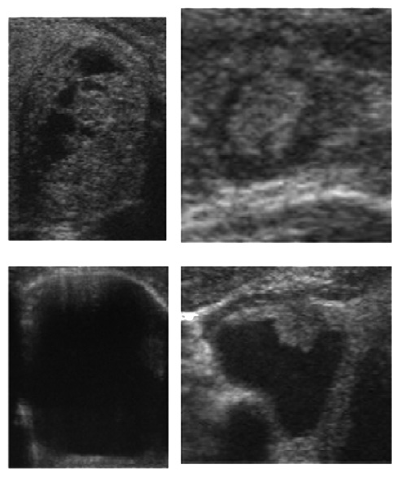
\includegraphics[width=0.40\textwidth]{2/figures/imagenes_ultrasonido_originales.png}
		\caption[Imágenes de ultrasonido de nódulos tiroideos]{Imágenes de ultrasonido de nódulos tiroideos. \\
		Fuente: \cite{pr_JERBI2023autoclassViTGAN}. \textit{Automatic classification of ultrasound thyroids images using vision transformers and generative adversarial networks}.}
		\label{2:fig210}
	\end{center}
\end{figure}


\subsection{Transfer Learning}
\cite{bk_geron2022handml} nos menciona que el Transfer Learning o Transferencia de Aprendizaje es un técnica usada en el campo de Deep Learning que permite el uso de algunas capas de un modelo ya definido y entrenado previamente en un nuevo modelo que necesite ser entrenado en una tarea similar al que se desarrolla el modelo original. Las capas destinadas al reuso son normalmente las más cercanas a la entrada o también conocidas como capas inferiores. El beneficio de usar esta técnica radica en dos puntos importantes: cantidad de datos requeridos y velocidad de entrenamiento del modelo; es decir, la cantidad de datos que se deben usar para entrenar un modelo de alto desempeño se reduce considerablemente, mientras que el tiempo requerido para terminar este proceso es menor comparándolo a si lo entrenaran desde cero.

Para que esta técnica funcione debidamente, las capas más cercanas a la salida, conocidas también como capas de alto nivel, deben ser reemplazadas, esto debido a que son más específicas de las tareas del modelo original. Esto también incluye a la capa final, ya que posiblemente no tenga la cantidad de salidas necesarias para completar satisfactoriamente la nueva tarea.

En la Figura \ref{2:fig211} se presenta de forma gráfica la técnica.

\begin{figure}[H]
	\begin{center}
		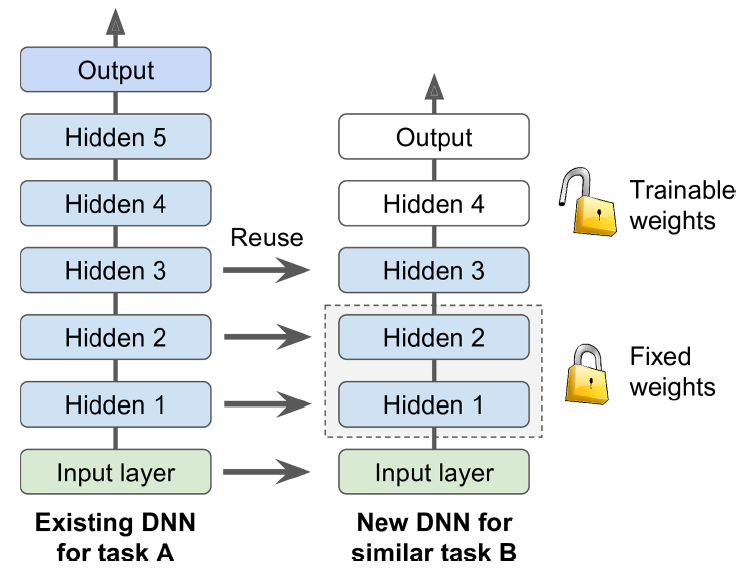
\includegraphics[width=0.70\textwidth]{2/figures/transfer_learning.PNG}
		\caption[Ejemplo de Transfer Learning]{Ejemplo de Transfer Learning. \\
		Fuente: \cite{bk_geron2022handml}. \textit{Hands-on machine learning with Scikit-Learn, Keras, and TensorFlow}.}
		\label{2:fig211}
	\end{center}
\end{figure}


\subsection{Data Augmentation}

Según \cite{bk_geron2022handml} el Aumento de Datos o Data Augmentation es una técnica de regularización que permite reforzar la cantidad de muestras en un conjunto de datos. Esto se realiza a través de la generación de nuevas instancias similares a los originales; es decir, las personas no deberían ser capaces de diferenciar una imagen generada de una del propio conjunto de datos.

Para generar estas nuevas muestras, normalmente se aplican diferentes transformaciones a las instancias del conjunto de datos original. Estas transformaciones pueden ser; por ejemplo, una simple rotación o recorte de la imagen, siempre y cuando no altere por completo su sentido como es el caso de voltear una imagen de texto de forma horizontal. 

El principal beneficio de esta técnica es que permite reducir el sobreajuste de los modelos entrenados. 

En la Figura \ref{2:fig212} se muestran algunas transformaciones que se pueden hacer al aplicar el Aumento de Datos. 

\begin{figure}[H]
	\begin{center}
		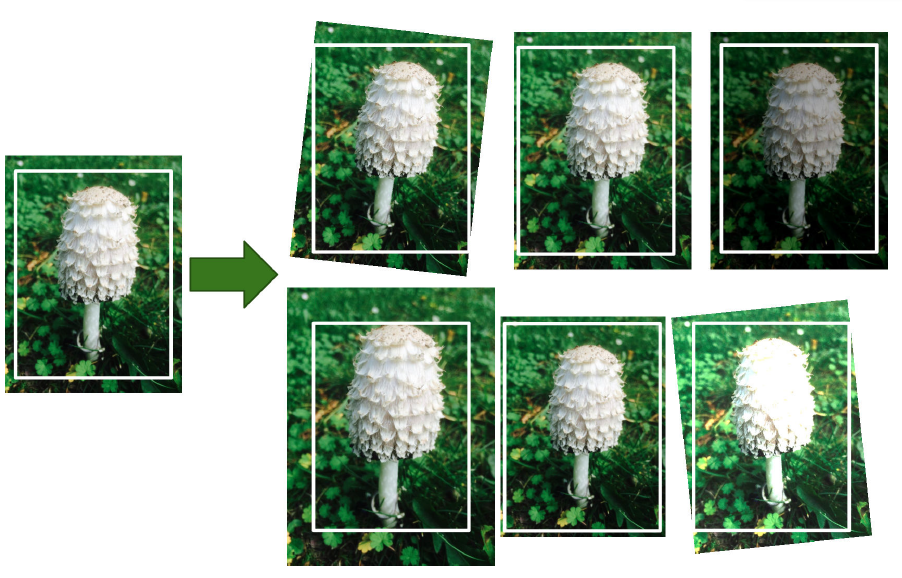
\includegraphics[width=0.85\textwidth]{2/figures/data_aug.PNG}
		\caption[Ejemplo de Data Augmentation]{Ejemplo de Data Augmentation. \\
		Fuente: \cite{bk_geron2022handml}. \textit{Hands-on machine learning with Scikit-Learn, Keras, and TensorFlow}.}
		\label{2:fig212}
	\end{center}
\end{figure}

\end{comment}